\chapter{Empregos}
\section{Introdução}
\par Os empregos são  vetores de indicações para a atividade econômica de um país, por isso, o governo federal realiza inúmeras pesquisas sobre os empregos formais e informais. Assim, tem-se o CAGED (Cadastro Geral de Empregados e Desempregados) que reune inúmeras informações sobre os empregos formais, sendo, admissão, desligamento, salários, funções, cargos, etc.
\par O CAGED é atualizado mensalmente pelo ministério do trabalho, gerando uma atualização destes dados para realização de pesquisas e prognósticos econômicos. Outro ponto, é que o CAGED abrange tanto a unidade federativa geral, como estados e municípios, gerando uma demonstração uniforme nos dados nacionais. Nos tópicos a seguir desta sessão de empregos, analise-se e estuda-se os dados sobre empregos formais referentes ao primeiro semestre de 2020.
\par Também usa-se os dados da PNAD Continua, para calcular a taxa de desemprego, ocupação, renda média dos trabalhadores. Utilizando esses conjuntos de dados será iniciado uma analise da situação do mercado de trabalho no estado do Tocantins, começando  o objetivo de se estudar o primeiro semestre de 2020 e fazendo comparativos com o primeiro semestre de 2019.

\begin{smbox}[label={labelbox},nameref={Empregos}]{Empregos}
O CAGED (Cadastro Geral de Empregados e Desempregados) tem um inicio da série em 1992 para o Brasil em geral, agora para os estados tem de inicio por volta de 1996, sempre feito pelo Ministério do Trabalho. Porém, um problema nacional é a nossa mudança de metodologias que ocorrem em decorrer desse período. O CAGED e divulgado todos os meses, por voltado dos dias 02 até o dia 10 do mês vigente.
\end{smbox}

\section{Saldo de Empregos}
\par Analisando os dados do saldo de emprego até o segundo trimestre. É de se visualizar o impacto da COVID-19 nos meses que o isolamento social teve uma maior latência.

\begin{figure}[h]
	\caption{Saldo de Empregos - Tocantins}
	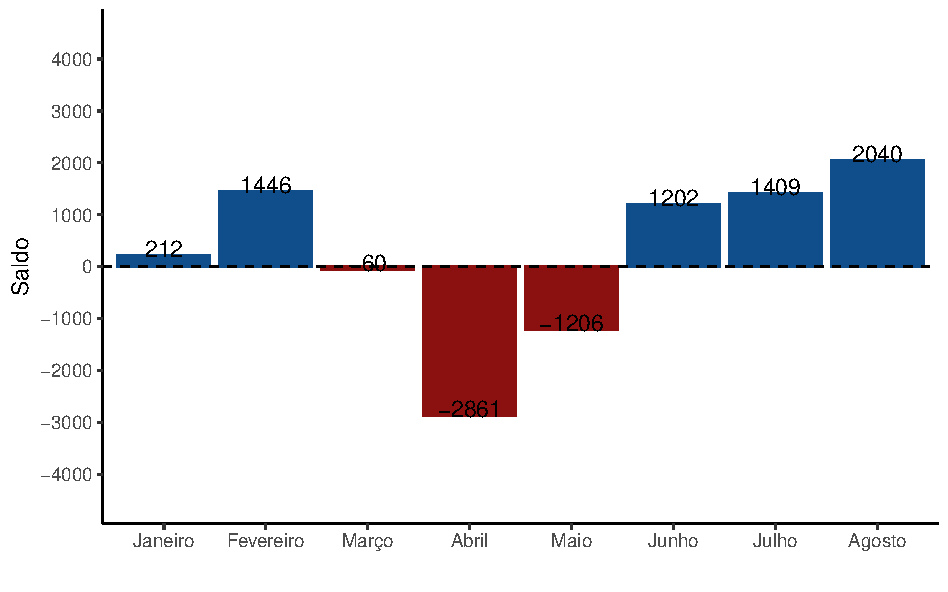
\includegraphics[width=\linewidth]{fig/Saldo de empregos - Tocantins.pdf}
	\source{Ministério do Trabalho}
	\notes{Note-se que já esta em curso uma recuperação dos empregos formais no estado tocantinense.}
\end{figure}

\par Analisando a situação tocantinense, observa-se que o impacto dos
empregos no Tocantins foram consideráveis, gerando uma perda total de -4.127. Um impacto preocupante, porém, a partir de um afrouxamento do isolamento social ocorre uma recuperação destes empregos nos meses seguintes.

\par Já no caso da Região Norte, compreendemos um movimento bem similar ao do Tocantins. Existe uma semelhança bem especifica no período de impacto que os empregos sofreram, muito similar ao caso tocantinense. Foram os efeitos causados pela pandemia e consequentemente o isolamento social.

\begin{figure}[h]
	\caption{Saldo de Empregos - Região Norte}
	\includegraphics[width=\linewidth]{fig/Saldo de Empregos - Região Norte.pdf}
	\source{Ministério do Trabalho}
	\notes{Note-se que já esta em curso uma recuperação dos empregos formais na região norte do Brasil, semelhante ao movimento tocantinense.}
\end{figure}
\newpage
\section{Saldo Trimestral - TO}
\par Produzindo uma análise por trimestres no Tocantins é observado que os empregos em estavam em uma crescente partindo do 1T até o 3T de 2019, porém no 4T acontece uma queda nesse ciclo de criação de empregos. Em 2020, estava havendo uma recuperação no mercado de trabalho, conforme relatado no 1T. Mas, no 2T tivemos o impacto do Covid-19, gerando uma grande perda de vagas formais.

\begin{figure}[h]
	\caption{Série de Empregos - Tocantins}
	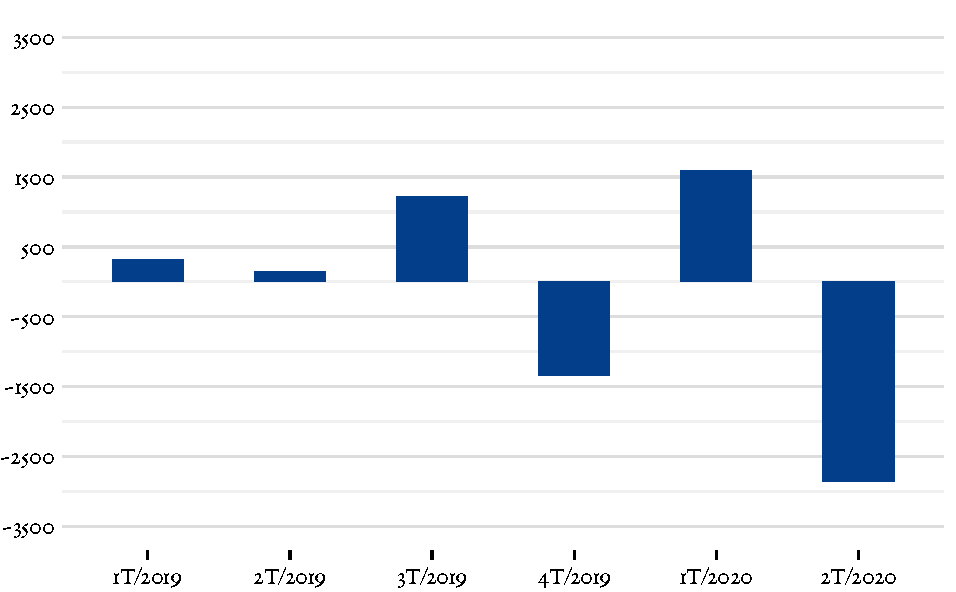
\includegraphics[width=\linewidth]{fig/Saldo por trimestre - Tocantins.pdf}
	\source{Ministério do Trabalho}
	\notes{Relação por trimestre a partir do 1T de 2019 para acompanhar o movimento que os empregos estão tendo.}
\end{figure}

\section{Saldo Trimestral - Região Norte}
\par O mesmo padrão ocorre na região norte. Menos no 1T de 2019, porque o estado do Tocantins teve números melhores do que a própria região norte, entretanto, a geração e perda de empregos formais é semelhante ao do estado tocantinense.

\begin{figure}[h]
	\caption{Série de Empregos - Região Norte}
	\includegraphics[width=\linewidth]{fig/Saldo por trimestre - Região Norte.pdf}
	\source{Ministério do Trabalho}
	\notes{Relação por trimestre a partir do 1T de 2019 para acompanhar o movimento que os empregos estão tendo.}
\end{figure}
\newpage

\section{Grau de instrução dos admitidos e demitidos}

\par Um ponto para se analisar é o nível de instrução dos admitidos e demitidos no Tocantins dentro do primeiro semestre de 2020, aponta-se qual o nível de formação dos admitidos do estado tocantinense.
\newpage
\begin{table}
	\caption{\label{tab:}Admitidos e Demitidos por Grau de Instrução}
	\centering
	\begin{tabu} to \linewidth {>{\raggedright\arraybackslash}p{4cm}>{\raggedleft}X>{\raggedleft}X}
		\toprule
		Instrução & Admitidos & Demitidos\\
		\midrule
		Analfabeto & 0.36\% & 0.34\%\\
		Até 5ª Incompleto & 2.63\% & 2.00\%\\
		5ª Completo Fundamental & 1.52\% & 1.72\%\\
		6ª a 9ª Fundamental & 3.89\% & 3.86\%\\
		Fundamental Completo & 5.74\% & 5.78\%\\
		\addlinespace
		Médio Incompleto & 6.66\% & 7.39\%\\
		Médio Completo & 66.70\% & 67.21\%\\
		Superior Incompleto & 3.97\% & 4.4\%\\
		Superior Completo & 7.67\% & 6.65\%\\
		Mestrado & 0.23\% & 0.17\%\\
		\addlinespace
		Doutorado & 0.07\% & 0.05\%\\
		Pós-Graduação completa & 0.55\% & 0.41\%\\
		\bottomrule
		\source{CAGED}
\end{tabu}
\end{table}

\par Um ponto interessante é a quantidade de pessoas com o ensino médio completo sendo admitidas, mostrando que o grau de empregos gerados no Tocantins é de nível médio e superior completo. Com o ensino médio correspondendo 66,63 ¨\% e com o ensino superior 8,50 \%.

\par Já nos desligamentos e o seu grau de instrução, é bem similar aos admitidos, no primeiro trimestre também é apresentado uma demissão maior com pessoas de ensino médio e também o médio incompleto com o superior completo. Dá pra se pensar que existe uma alta rotatividade de vagas referente ao ensino médio.

\section{Setores de contratações e demissões.}
\par Um ponto crucial para entender o contexto dessas admissões e demissões é compreender os setores que mais contratam e consequentemente também demitem. Por isso, é usado a CNAE (Classificação Nacional de Atividades Econômicas), pois realizam esses cortes nos setores econômicos. Uma particularidade que acontece na situação tocantinense é que verificado uma falta de dados para todos os setores.

\newpage

\begin{table*}[h]
\caption{Admitidos e Demitidos por Setor}
\centering
\begin{tabu} to \linewidth {>{\raggedright}X>{\raggedleft}X>{\raggedleft}X}
\toprule
Setor & Admitidos & Demitidos\\
\midrule
Agricultura, Pecuária, Produção Florestal, Pesca e Aquicultura & 2562 & 2285\\
Indústrias Extrativas & 289 & 117\\
Indústrias de Transformação & 2827 & 2825\\
Eletricidade e Gás & 57 & 134\\
Água, Esgoto, Atividades de Gestão de Resíduos e Descontaminação & 116 & 104\\
\addlinespace
Construção & 4583 & 3622\\
Comércio, Reparação de Veículos Automotores e Motocicletas & 8609 & 10559\\
Transporte, Armazenagem e Correio & 2142 & 2240\\
Alojamento e Alimentação & 1242 & 1762\\
Informação e Comunicação & 397 & 376\\
\addlinespace
Atividades Financeiras, de Seguros e Serviços Relacionados & 191 & 154\\
Atividades Imobiliárias & 109 & 113\\
Atividades Profissionais, Científicas e Técnicas & 1071 & 926\\
Atividades Administrativas e Serviços Complementares & 2720 & 3165\\
Administração Pública, Defesa e Seguridade Social & 5 & 8\\
\addlinespace
Educação & 977 & 916\\
Saúde Humana e Serviços Sociais & 1320 & 999\\
Artes, Cultura, Esporte e Recreação & 101 & 127\\
Outras Atividades de Serviços & 602 & 751\\
\bottomrule
\end{tabu}
\end{table*}

\par No primeiro semestre de 2020, as admissões se concentraram no setor do comércio. Demonstrando o poder do setor na na economia tocantinense, abrindo 5.794 vagas no período semestral. É de se estudar que o Tocantins é um estado novo, mas com uma economia dinâmica e com padrões de movimentos bruscos nos setores de empregos. 
\par Assim, o saldo por setores no primeiro semestre é composto pelos seguintes números:

\begin{figure}[h]
	\caption{Saldo por setores - Tocantins}
	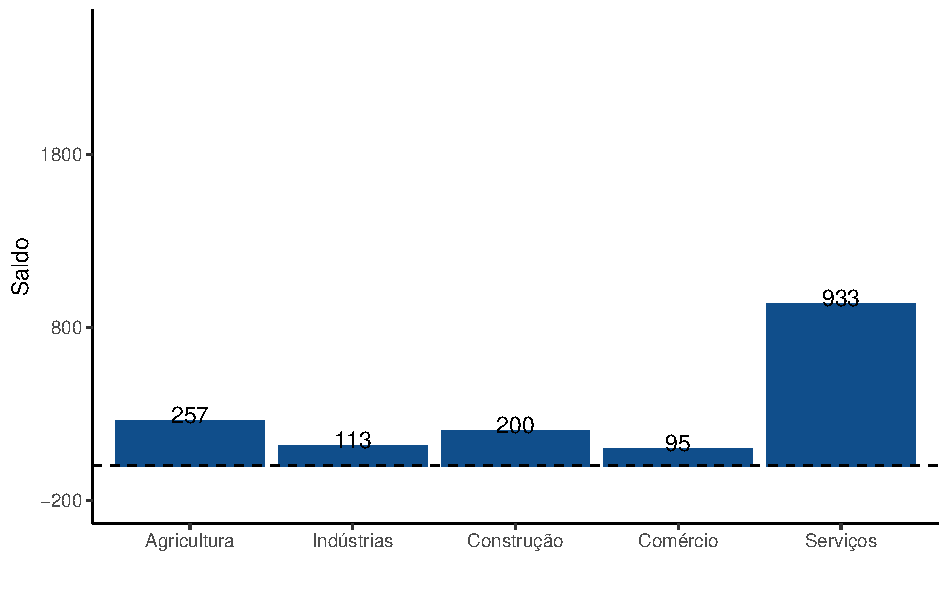
\includegraphics[width=\linewidth]{fig/Saldo por setores.pdf}
	\source{Ministério do Trabalho}
	\notes{Relação do primeiro semestre de 2020 por setores.}
\end{figure}
\newpage
\section{Perfil de Idade}

\par Nessa sessão expõe o perfil de idade dos contratados e demitidos.


\par Nos admitidos apresenta-se a noção de que pelo primeiro corte de 14-34 anos, ocorre uma maior contratação.
\newpage
\begin{table}
\caption{Admitidos e Demitidos por Idade}
\centering
\begin{tabu} to \linewidth {>{\raggedright}X>{\raggedleft}X>{\raggedleft}X}
\toprule
Idade & Admitidos & Demitidos\\
\midrule
14-34 & 20627 & 20881\\
35-65 & 9251 & 11061\\
65+ & 32 & 95\\
\bottomrule
\end{tabu}
\end{table}

\par Os desligamentos seguem o mesmo movimento, é possível analisar que existe uma variabilidade de contratações e demissões para a população mais jovem. E nesse primeiro trimestre isso foi corroborado. 

\begin{figure}[h]
	\caption{Saldo por faixa etária - Tocantins}
	\includegraphics[width=\linewidth]{fig/Saldo de empregos por faixa etária.pdf}
	\source{Ministério do Trabalho \\ Elaborado por: PET-Economia}
	\notes{Relação do primeiro trimestre de 2020 por idade.}
\end{figure}

\par No primeiro semestre de 2020, observa-se que indivíduos com mais de 35 anos, tiveram mais demissões do que indivíduos com idades inferiores.

\section{Genêro}
\par Outro parâmetro para a realização da exposição destes saldos é ter uma visão por gênero, entender como o mercado de trabalho está funcionando para homens e mulheres. 

\begin{table}
\caption{Admitidos e Demitidos por Sexo}
\centering
\begin{tabu} to \linewidth {>{\raggedright}X>{\raggedleft}X>{\raggedleft}X}
\toprule
Sexo & Admitidos & Demitidos\\
\midrule
Homem & 20849 & 20667\\
Mulher & 9071 & 10519\\
\bottomrule
\end{tabu}
\end{table}

\begin{figure}[h]
	\caption{Saldo por gênero - Tocantins}
	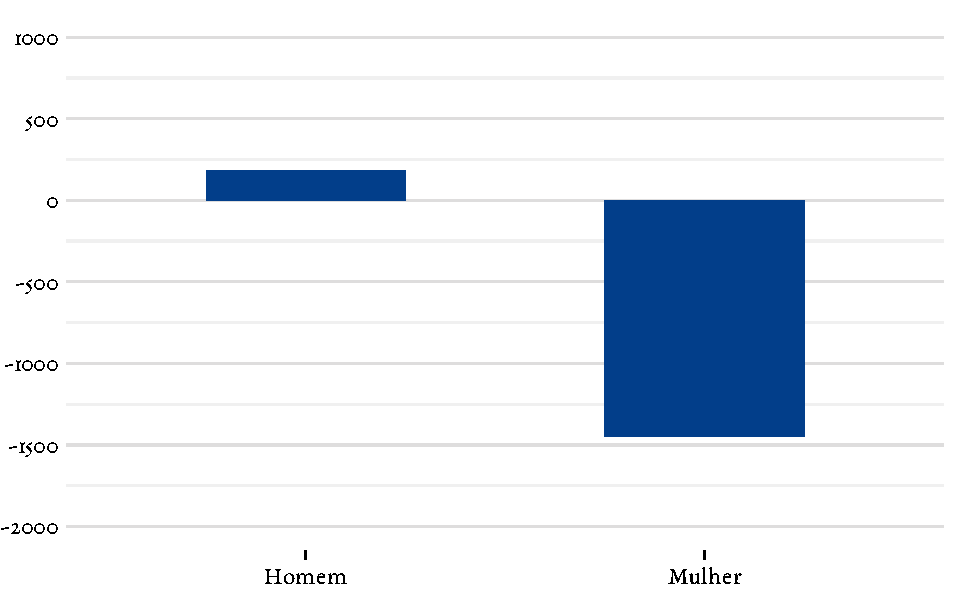
\includegraphics[width=\linewidth]{fig/Saldo por genero.pdf}
	\source{Ministério do Trabalho}
	\notes{Relação do primeiro trimestre de 2020 por gênero.}
\end{figure}
\newpage
\par No primeiro semestre de 2020, as mulheres conseguiram manter os seus empregos, mesmo havendo menos contrações do que os homens, um ponto interessante desse primeiro trimestre é de como as mulheres conseguiram manter os seus empregos formais de forma mais visíveis do que os homens.


\begin{smbox}[label={labelbox},nameref={Desigualdade por gênero}]{Desigualdade por gênero}
	Já é um tópico bem usual que o mercado de trabalho formal é um quanto desigual para as mulheres, existe uma vasta literatura sobre desigualdades salarias, vagas de empregos, oportunidades, etc. \cite{bibCotrim2020desigualdade} e \cite{bibHaussmann2018desigualdades} fazem um bom estudo e mais aprofundado sobre estas desigualdades.
\end{smbox}

\section{Etnia}
\par Agora, seguindo a análise desse semestre, é demonstrado os dados referentes a etnia desses indivíduos.

\begin{figure}[h]
	\caption{Saldo por gênero - Tocantins}
	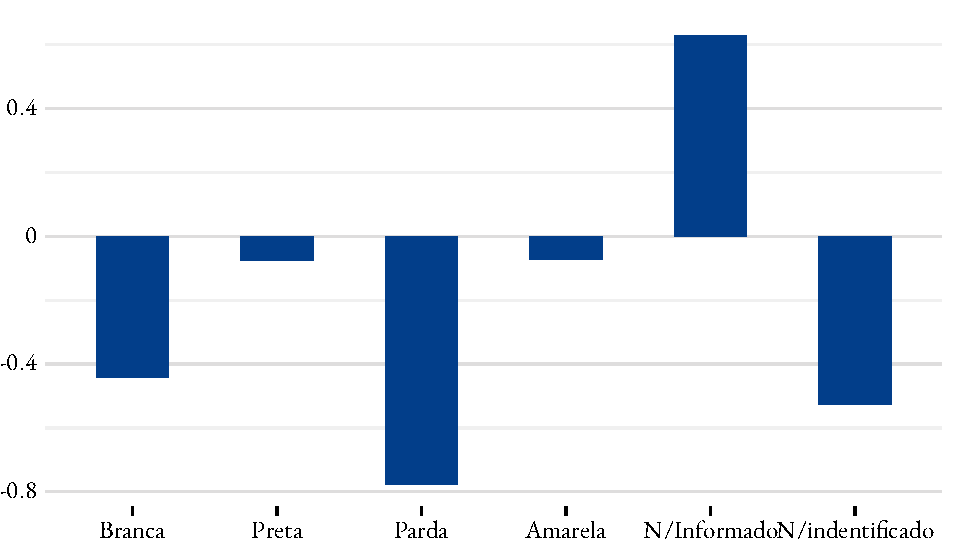
\includegraphics[width=\linewidth]{fig/Saldo por etnia.pdf}
	\source{Ministério do Trabalho}
	\notes{Relação do primeiro trimestre de 2020 por etnia.}
\end{figure}
\newpage
\par De uma forma contundente, é de se analisar que a movimentação dos empregos é de complexa. Por exemplo, a uma quantidade grande de pessoas que não declaram sua etnia e quando declaram, é majoritariamente parda. Finalizando essa parte dos dados oriundos do CAGED, um adendo importante para se entender é que as áreas que ocorre as maiores contratações são auxiliar de escritório, operador de caixa, faxineiro, vendedor de comércio varejista, servente de obras, motorista de caminhão e assistente administrativo

\section{Taxa de Desemprego}

\par A taxa de desemprego é fornecida pela PNAD-C/IBGE (Pesquisa Nacional por Amostra de Domicílios). É divulgada pelo IBGE de forma trimestral e para todos os estados da federação, ela calcula a população ocupada pela desocupada, assim, gerando a nossa taxa de desemprego. A seguir, é exposto a atual taxa de desemprego tocantinense.

\begin{figure}[h]
	\caption{Taxa de desemprego - Tocantins}
	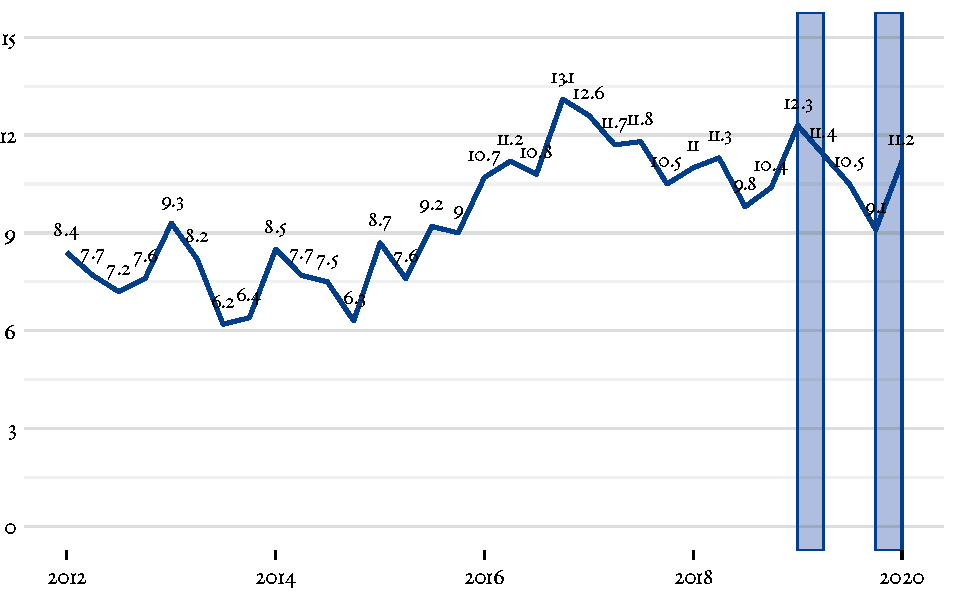
\includegraphics[width=\linewidth]{fig/taxa de desemprego - Tocantins.pdf}
	\source{PNAD/IBGE}
	\notes{Relação taxa de desemprego primeiro trimestre de 2020.}
\end{figure}

\par A taxa de desemprego no Tocantins estava num movimento de queda a partir do primeiro trimestre de 2019, porém, a partir do 4T de 2019 até o 1T de 2020 ocorre um movimento de elevação da taxa de desemprego.

\section{Seguro Desemprego}

\par Outro termômetro claro para o setor de empregos são os pedidos seguro-desemprego, que é uma politica macroeconômico para gerar uma segurança branda para o trabalhador recém demitido. Num contexto mais claro, significa que se ocorre uma elevação dos pedidos seguro desemprego, significa que o mercado de trabalho não está em um bom funcionamento. O inverso é bem intuitivo, se a poucos pedidos é uma reação a um bom momento econômico.

\begin{figure}[h]
	\caption{Pedidos seguro desemprego - Tocantins}
	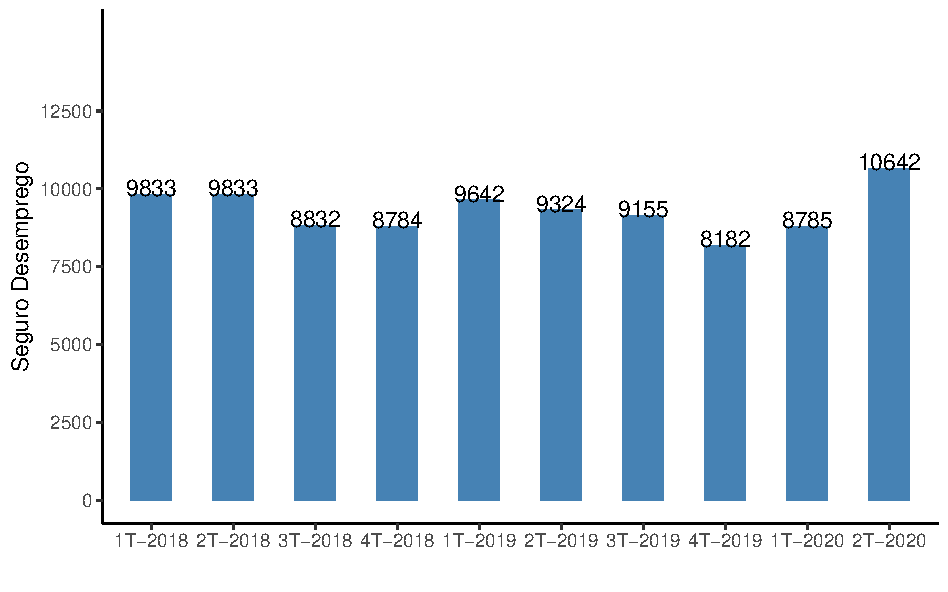
\includegraphics[width=\linewidth]{fig/Pedidos seguro desemprego.pdf}
	\source{Ministério do Trabalho}
	\notes{Relação pedidos seguro desemprego  primeiro trimestre de 2020.}
\end{figure}

\par Fazendo uma comparação com a taxa de desemprego, é apresentado a noção de que a taxa se eleva e gera um aumento nos pedidos de seguro desemprego, uma demonstração clara de como a taxa é crucial para a avaliação macroeconômica. Realiza-se uma regressão para definir o quão importante é a taxa de desemprego em relação ao seguro desemprego, para o seguinte caso:

\begin{figure}[h]
	\caption{Relação taxa de desemprego x pedidos seguro desemprego}
	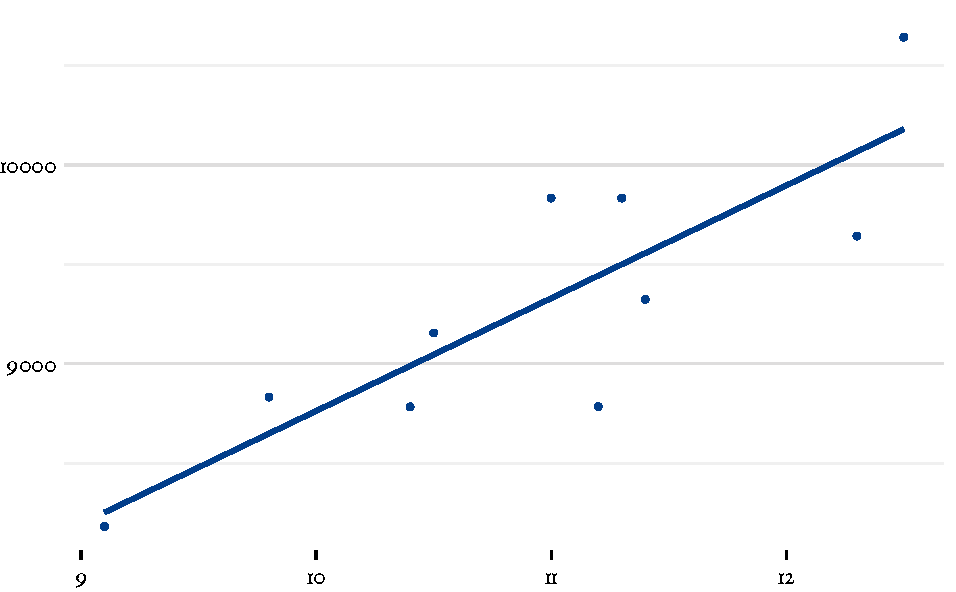
\includegraphics[width=\linewidth]{fig/Relação taxa desemprego x seguro desemprego.pdf}
	\source{Ministério do Trabalho}
	\notes{Relação pedidos seguro desemprego com a taxa de desemprego  primeiro trimestre de 2020.}
\end{figure}

\begin{smbox}[label={labelbox},nameref={Desigualdade por gênero}]{Regressão linear}
	Usamos uma técnica acima para provar a correlação da taxa de seguro desemprego e pedidos de seguro desemprego. Essa técnica é a regressão linear simples, quando existe apenas uma variável resposta e uma variável explicativa, por isso chamamos de regressão linear simples. A formula é determinada por $y = \alpha + \beta x$ e $\beta = \overline{y} - \overline{\alpha x}$.
	\\
	Por fim, utilizando um processo econométrico vemos que a relação é forte, para se ter a ideia o \textbf{R} que é referente ao processo de correlação nos aponta um número de 0,70 (quanto mais próximo de 1 for, mais forte é a relação) e o \textbf{R}$^{2}$ é de 0,66. Ou seja, essa correlação é muito forte. 
\end{smbox}

\section{População Ocupada}

\par Outro ponto crucial é a população economicamente ativa ocupada, é uma demonstração da população economicamente ativa que está trabalhando.

\begin{figure}[h]
	\caption{População Ocupada - Tocantins}
	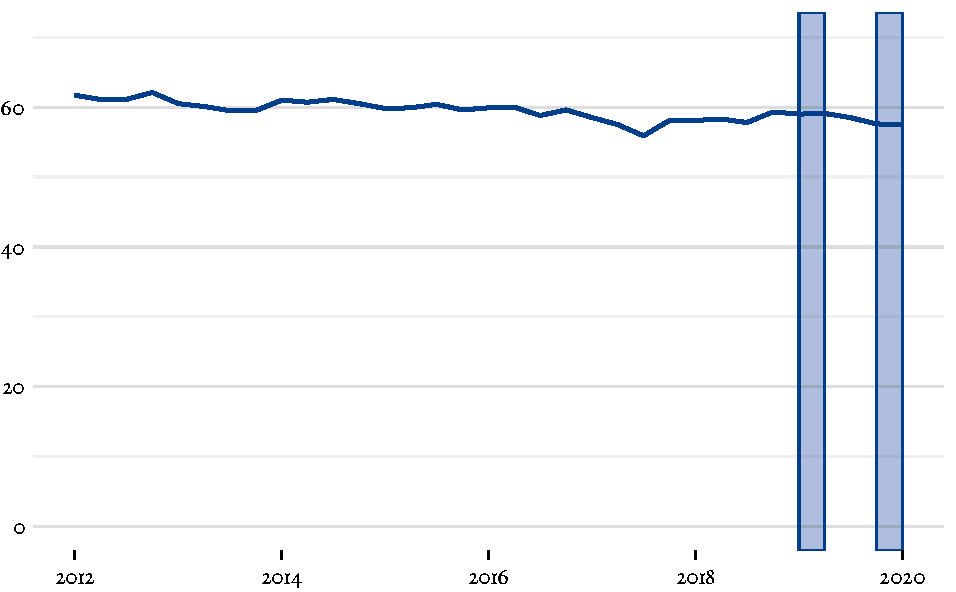
\includegraphics[width=\linewidth]{fig/População Ocupada.pdf}
	\source{PNAD/IBGE}
	\notes{Relação taxa de ocupação primeiro trimestre de 2020.}
\end{figure}

\par  A taxa de ocupação tocantinense é bem estável pelos dados, sempre na faixa de 60\%, o que demonstra uma certa estabilidade dessa população. Comparando a taxa do 1T de 2019, foi de 59\% e no prímeiro 1T de 2020 foi de 57,5\%. Uma queda percentual da população ocupada.

\section{Rendimento Médio}

\par O rendimento médio do Tocantins é derivado dos rendimentos dos trabalhadores, nele, é possível de se pensar na renda que esses agentes produzem. É fruto do trabalho da nossa população ocupada, sejam trabalhos principais ou habituais. 

\begin{figure}[h]
	\caption{Rendimento médio - Tocantins}
	\includegraphics[width=\linewidth]{fig/Rendimento médio - Tocantins.pdf}
	\source{PNAD/IBGE}
	\notes{Relação dos rendimentos médios no primeiro trimestre de 2020.}
\end{figure}

\par A renda dos trabalhadores tocantinenses está na faixa dos R\$ 1.700,00 e R\$ 1.800,00 por alguns anos, no primeiro período de 2019, a renda foi de R\$ 1.807,00 e no primeiro trimestre de 2020, foi de R\$ 1.867. Ou seja, a partir do primeiro trimestre de 2019, houve um ganho de renda muito considerável. É claro que o rendimento médio comparado com outros estados brasileiros é bem baixa, iremos comparar com a renda da região norte e do Brasil em geral.

\begin{figure}[h]
	\caption{Rendimento médio - Região Norte}
	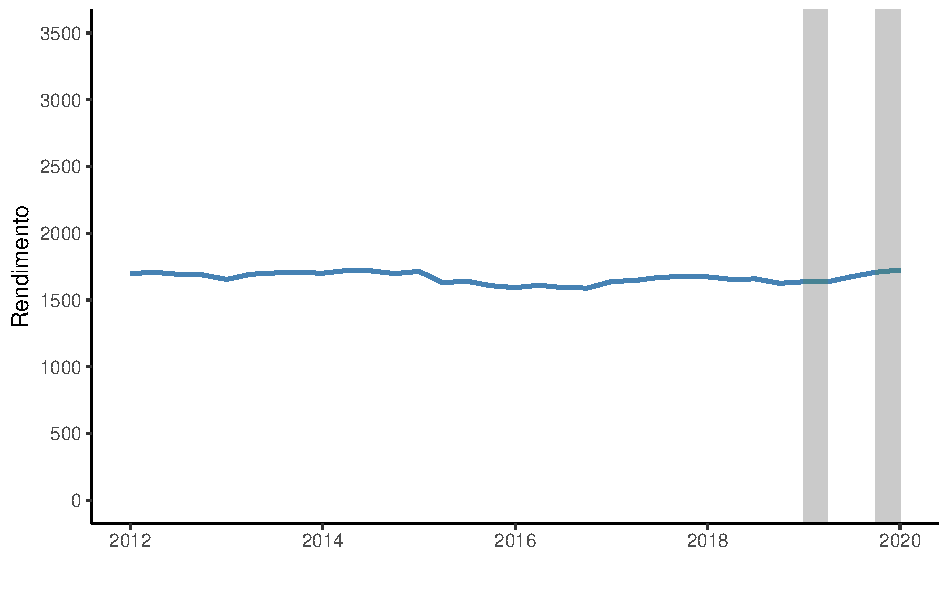
\includegraphics[width=\linewidth]{fig/Rendimento médio - Região Norte.pdf}
	\source{PNAD/IBGE}
	\notes{Relação dos rendimentos médios no primeiro trimestre de 2020.}
\end{figure}

\par A região Norte tem uma renda média menor que a do estado do Tocantins, por exemplo, no primeiro trimestre de 2019, a renda nortenha foi de R\$ 1.637,12 e no primeiro trimestre de 2020 o resultado de R\$ 1.725,25. Houve um aumento de renda desses trabalhadores, mas, abaixo do Tocantins.

\begin{figure}[h]
	\caption{Rendimento médio - Brasil}
	\includegraphics[width=\linewidth]{fig/Rendimento médio - Brasil.pdf}
	\source{PNAD/IBGE}
	\notes{Relação dos rendimentos médios no primeiro trimestre de 2020.}
\end{figure}

\par No caso da renda média nacional, acontece um "gap" maior, a renda nacional no primeiro trimestre de 2019 foi de R\$ 2.159,51 e no 1T de 2020, foi de R\$ 2.261,29. A região Norte e o estado do Tocantins estão com um nível de renda menor que o Brasil no geral, mas, a renda média nacional é puxada por regiões que o desenvolvimento é maior e por consequência, uma maior produtividade. Os eixos nacionais (Sul e Sudeste) tem os seus níveis de renda maiores.
